\section{ Introduction }

\emph{Data compression}, \emph{source coding}, or \emph{bit-rate reduction} involve encoding information using fewer bits than the original representation.

\subsection{ Introduction to the problem }

Data compression is achieved by different types of algorithms, but in order
to study it formally we use a formal definition of a data compression scheme. 
First, we describe an algorithm which operates on words - 
in our case, Lempel-Ziv 78.
Then, we introduce a probabilitic model representing
the data to be compressed, which allows us to quantify
the efficiency of the algorithm.


\subsubsection{ Compression algorithm : Lempel-Ziv 78 }

\begin{definition}
    A \emph{compression algorithm} is a pair of functions on
    words $(\mathcal{C}, \mathcal{D})$ - compressor and 
    decompressor.
\end{definition}

\begin{definition}
    \label{def:lossless}
    A \emph{lossless} compression algorithm decompresses 
    the exact same data that was compressed in the first place.
\end{definition}

\begin{rmk}
    We will not describe the decompression part of 
    our algorithms, considering that the possibility
    of decompression is obvious in the case of LZ78.
\end{rmk}

In general, Lempel-Ziv algorithms dictionary-based scheme
which exploit previously seen patterns and redundancy to 
save off coding space. 
The Lempel-Ziv'78 (LZ'78) that partitions a sequence into 
phrases or blocks of variable size such that a new phrase
is the shortest substring not seen in the past as a phrase. 
Every such phrase is encoded by the index of its prefix 
appended by a symbol; thus the LZ'78 code contains the 
pairs \verb|(pointer, symbol)|.
For example, the string 
\centers{11001010001000100} of length 17 is parsed
as 
\centers{(1)(10)(0)(101)(00)(01)(000)(100)}
which can be be 
encoded in the following digital search tree:

\centers{
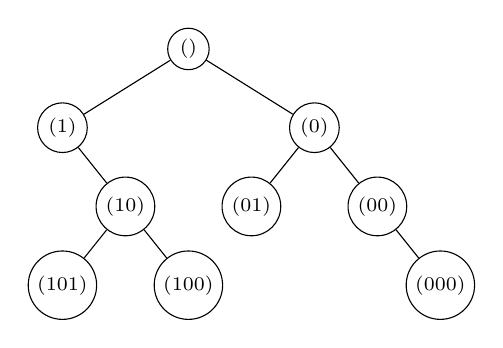
\begin{tikzpicture}[
    level 1/.style={level distance=10mm,sibling distance=32mm},
    level 2/.style={level distance=10mm,sibling distance=16mm},
    level 3/.style={level distance=10mm,sibling distance=16mm},
    font=\scriptsize,inner sep=2pt,every node/.style={draw,circle,minimum size=3ex}]
  ]
  \node {()}
    child {node {(1)}
        child[missing]
        child {node {(10)}
            child {node {(101)}}
            child {node {(100)}}
        }
    }
    child {node {(0)}
        child {node {(01)}}
        child {node {(00)}
            child[missing]
            child {node {(000)}}
        }
    }
        ;
\end{tikzpicture}
}




\subsubsection{ Probabilistic models }

\begin{df}
    \label{def:source}
    Let $\mathcal{A}$ be an alphabet.
    An \emph{information source} is a one-sided infinite sequence of random
    variables $(X_k)_{k=1}^{\pinf}$ with each $X_k$ 
    having values in $\mathcal{A}$.
\end{df}

\begin{rmk}
    \label{rmk:sequence}
    Each realization of an information source is called a 
    \emph{sequence} or \emph{word}.
\end{rmk}

\begin{rmk}
    \label{rmk:source}
    \emph{Defining} the law of the $X_k$ produces out different
    models for data generation which can be studied mathematically
    and \emph{simulated}.
\end{rmk}

\begin{df}
    \label{def:memoryless}
    A \emph{memoryless source} is an \emph{information source}
    for which the $X_k$ are mutually independent, following
    the uniform law on $\mathcal{A} = \{ a_1, \dots, a_V \}$ :
    \centers{$
        \proba{} \left( X_k = a_k \right) = p_k 
        \qquad \textmd{with } \,\Sum{i=1}{V} \,p_i = 1
    $}
\end{df}

\begin{rmk}
    \label{rmk:memoryless}
    This is the simplest information source and it has been 
    studied successfully in the past, but it is not a realistic 
    model. We replace it with the following Markov model whenever 
    possible.
\end{rmk}

\begin{df}
    \label{def:markov}
    A \emph{Markov source} is an \emph{information source}
    with a Markov dependency between successive symbols.
\end{df}

\begin{df}
    \label{def:markovorder}
    A \emph{Markov source of order $r$} is a Markov source
    for which each symbol apparition depends on the previous 
    $r$ symbols.
\end{df}

\begin{rmk}
    \label{rmk:markov2}
    We will study Markov sources of order 1 - where each
    symbol simply depends on the previous one. This is 
    general enough, as Markov sources of superior order
    can be simulated by expanding the alphabet and 
    using a Markov source of order 1.
\end{rmk}

\subsubsection{ Entropy }

    In this study, we consider only two information sources:
    the \emph{memoryless} and the \emph{Markov} source.
    For the Markov source, we consider that there exists a 
    \emph{stationary distribution}.

    \begin{df}
        \label{def:entropy}
        The \emph{entropy} of an information is the average
        rate at which information is produced by a probabilistic
        source of information.
    \end{df}

    \begin{prop}
        \label{prop:memorylessentropy}
        The entropy of a \emph{memoryless source} on 
        alphabet $\mathcal{A} = \{ a_1,\dots,a_V \}$ is:
        \centers{$ \Sum{i=1} p_i \log p_i$}
    \end{prop}

    \begin{prop}
        \label{prop:markoventropy}
        The entropy of a \emph{Markov source} with probability
        $(p_{i j})_{(i, j) \in { \{1,\dots,V\} }^2} $ and a 
        stationary distribution $(\pi_1, \dots, \pi_V)$ is:
        \centers{$ h = \Sum{i=1} \pi_i \Sum{j=1} p_{i j} \log p_{i j} $}
    \end{prop}

    
    The entropy gives a lower bound on the compression 
    ratio of lossless algorithms. Furthermore, in our
    case, for a memoryless or Markov source, the compression
    tends asymptotically to the entropy of the source:
    

    \begin{prop}
        \label{prop:lowerbound}
        \centers{$\underset{\limt}{n\rightarrow\pinf}\f{C_n}{n} = h$}
    \end{prop}


\subsubsection{ Probabilistic analysis }

Under this context, we can define and conduct a thorough
analysis of several random variables with different meanings
regarding the effectiveness of compression.

\begin{nota}
    \label{nota:universe}
    Let $n$ be an integer - the size of the considered words.
    Defining $\Omega_n$ the set of words of size $n$ on alphabet
    $\mathcal{A}$. Each word being an event, a natural probability
    space is given by considering the output of size $n$ of a Markov
    source.
\end{nota}

\begin{rmk}
    \label{rmk:probaspace}
    We will now study random variables defined 
    on this probability space. 
\end{rmk}

\begin{nota}
    \label{nota:output}
    $W_n$ denotes words of size $n$ output by a given Markov source.
\end{nota}

\begin{nota}
    \label{nota:numberphrases}
    The \emph{number of phrases} used to compress words of size $n$ ($W_n$) with
    LZ78 is given by $M_n(W_n)$ or simply $M_n$.
\end{nota}

\begin{rmk}
    \label{rmk:numberphrases}
    This is one of the most important variables to consider because,
    as it will appear shortly, it is closely tied to the \emph{compression 
    ratio} of LZ78.
\end{rmk}

\begin{df}
    \label{df:codelength}
    The \emph{codelength} is the \emph{number of bits} required 
    to encode the LZ78-compressed version of a word, denoted by $C(W_n)$ or $C_n$.
\end{df}

\begin{df}
    \label{df:compratio}
    The \emph{compression ratio} for words of size $n$ is the ratio between the 
    codelength and initial size of a word, $\f{C(W_n)}{|W_n|} = \f{C_n}{n}$.
\end{df}

\begin{rmk}
    \label{rmk:asymptotic}
    We focus now, as stated in the title of this report, on the asymptotical behavior - 
    for $n \rightarrow \pinf$ - of the compression ratio. Certainly this gives us 
    information about real-world compression, as files on our computer often attain
    large numbers when measured in bits. However, this assumption can be nuanced.
    For example, the speed of convergence towards this asymptotic behavior can make 
    a non-negligible difference in real-world application, as we will see later on
    when we talk about the difference between LZ'77 and LZ'78 and Optimal Parsing.
\end{rmk}



\subsection{ Theorems and Goals }

    There is a number of interrogations and results that surround
    the LZ'78 compression scheme, and that have been doing so for 
    some time now. These were proven for the simplistic memoryless
    source model which will allow us to formulate these as 
    theorems for memoryless sources. But the more interesting case
    of Markov sources has all these theorems become conjectures.
    My first job was to simulate the process and output visualizations
    that would disprove or make these results seem more likely.

    \begin{th}
        \label{th:clt}
        For memoryless source
    \end{th}
